\documentclass[11pt]{article}
\usepackage{geometry}                % See geometry.pdf to learn the layout options. There are lots.
\geometry{a4paper}                   % ... or a4paper or a5paper or ... 
\usepackage{graphicx}
\usepackage{amsmath}
\usepackage{amssymb}
\usepackage{epstopdf}
\usepackage{verbatim}
\usepackage{url}
\usepackage{floatrow}
\usepackage{listings}
\usepackage{hyperref}
\newfloatcommand{capbtabbox}{table}[][\FBwidth]


\ifx\release\undefined
    \newcommand{\solution}[1]{{#1}}
\else
    \newcommand{\solution}[1]{{}}
\fi

\newcommand{\vect}[1]{\boldsymbol{#1}}
\newcommand{\mat}[1]{\boldsymbol{#1}}

\DeclareGraphicsRule{.tif}{png}{.png}{`convert #1 `dirname #1`/`basename #1 .tif`.png}


\title{Machine Learning Assignment 2: Neural Networks}
\author{\textbf{Name: Krunal Rathod | Email: krunal.rathod@usi.ch}}
\date{}                                           

\begin{document}
\maketitle 

\begin{list}{{\bf Question \arabic{enumi}}}
{\usecounter{enumi}
\setlength{\listparindent}{0mm}
\setlength{\leftmargin}{0mm}}


\item (20 points). Gradients of Loss Function \\

Given a two-layer neural network defined by the equation:
\[ y_k := w^{(2)} \cdot f(x_k \cdot W^{(1)} + b^{(1)})^T \cdot w^{(2)} + b^{(2)} \]

The values of the input vectors \(x_k\) (summarized in the matrix \(X\)), targets \(t_k\) (summarized in the vector \(t\)), weights \(W^{(1)}\) and \(w^{(2)}\), as well as biases \(b^{(1)}\) and \(b^{(2)}\) are given.

The function \(f\) is the ReLU nonlinearity. The loss of the model is:
\[ L := \frac{1}{2} \sum_{k=1}^{4} (y_k - t_k)^2 \]

\textbf{Forward Pass:}
\begin{align*}
    z^{(1)} &= X \cdot W^{(1)} + b^{(1)} \\
    h &= \text{ReLU}(z^{(1)}) \\
    y_k &= w^{(2)} \cdot h^T \cdot w^{(2)} + b^{(2)}
\end{align*}

\textbf{Loss Calculation:}
\[ L := \frac{1}{2} \sum_{k=1}^{4} (y_k - t_k)^2 \]

\textbf{Backward Pass:}
\begin{align*}
    \frac{\partial L}{\partial w^{(2)}} &= \sum_{k=1}^{4} (y_k - t_k) \cdot h \\
    \frac{\partial L}{\partial b^{(2)}} &= \sum_{k=1}^{4} (y_k - t_k) \\
    \frac{\partial L}{\partial W^{(1)}} &= X^T \cdot \left( \sum_{k=1}^{4} (y_k - t_k) \cdot w^{(2)} \cdot \text{ReLU}'(z^{(1)}) \right) \\
    \frac{\partial L}{\partial b^{(1)}} &= \sum_{k=1}^{4} (y_k - t_k) \cdot w^{(2)} \cdot \text{ReLU}'(z^{(1)})
\end{align*}

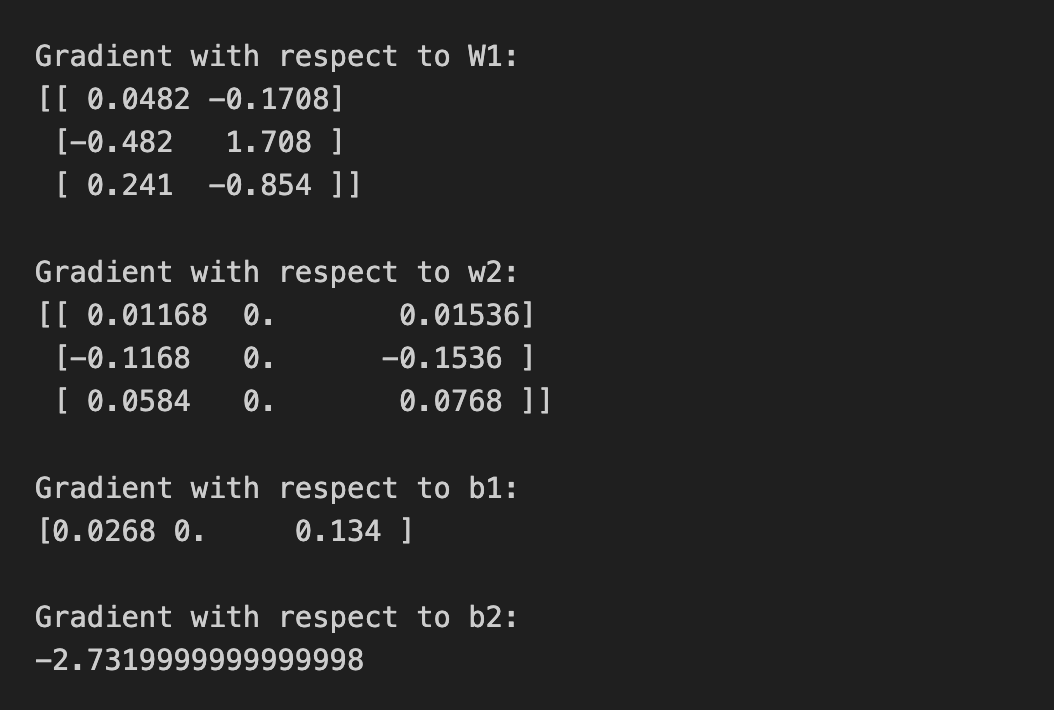
\includegraphics[width=16cm]{gradients.png}


\item (15 points). Softmax+Crossentropy \\

The Softmax function for the $i$-th element is given by:\\
\[
\text{Softmax}(y_i) = \frac{\exp(y_i)}{\sum_j \exp(y_j)}
\]

The Softmax+Crossentropy loss function is given by:\\
\[
E = - \sum_k t_k \log\left(\frac{\exp(y_k)}{\sum_i \exp(y_i)}\right)
\]

Now, let's calculate the gradient \(\frac{\partial E}{\partial y_{i}}\)
\[\frac{\partial E}{\partial y_{i}}=-\frac{\partial}{\partial y_{i}}\left(\sum_{k}t_{k}\log\left(\frac{\exp(y_k)}{\sum_i \exp(y_i)}\right)\right)\]

Firstly, differentiate the logarithm term:

\[\frac{\partial}{\partial y_{i}}log\left(\frac{exp(y_{k})}{\sum_{j}exp(y_{j})}\right)=\frac{\partial}{\partial y_{i}}\left(log(exp(y_{k}))-log\left(\sum_{j}exp(y_{j})\right)\right)\]

1. If \(i\ne k\)

                    \[=\frac{\partial}{\partial y_{i}}\left(0-log\left(\sum_{j}exp(y_{j}))\right)\right)=-\frac{\exp(y_{i})}{\sum_{j}exp(y_{j})}\]

2.                  If \(i=k\)
                    \[=\frac{\partial}{\partial y_{i}}\left(log(exp(y_{k}))-log\left(\sum_{j}exp(y_{j})\right)\right)=1-\frac{\exp(y_{i})}{\sum_{j}exp(y_{j})}\]

Now, summing over k in the expression for \(\frac{\partial E}{\partial y_{i}}\)

\[\frac{\partial E}{\partial y_{i}}=-\sum_{k}t_{k}\left(\delta_{ik}-\frac{\exp(y_{i})}{\sum_{j}exp(y_{j})}\right)\]


Now, consider the case where the target vector t is a one-hot vector (only one element is 1) , say~t_{k}=\delta_{ik}\)

\[\frac{\partial E}{\partial y_{i}}=-\sum_{k}\delta_{ik}\left(\delta_{ik}-\frac{\exp(y_{i})}{\sum_{j}exp(y_{j})}\right)\]

Simplifying further, we get:

\[\frac{\partial E}{\partial y_{i}}=-\left(1-\frac{\exp(y_{i})}{\sum_{j}exp(y_{j})}\right)=\frac{\exp(y_{i})}{\sum_{j}exp(y_{j})}-1\]

So, the simplified expression for \(\frac{\partial E}{\partial y_{i}}\) when the target is a one-hot vector is:

\[\frac{\partial E}{\partial y_{i}}=Softmax(yi) - 1\]




\item (15 points).  Gradient Descent Convergence \\


To ensure convergence in gradient descent, it's important to choose a suitable learning rate (\(\eta\)). The learning rate controls the size of the steps taken during each iteration, and if it's too high, the algorithm might overshoot the minimum, leading to divergence. The given function is \(f(x) = 5x^2 + 2\), and the gradient is \(f'(x) = 10x\). The update rule for gradient descent is \(x_{n+1} = x_n - \eta f'(x_n)\). To find the range of values for \(\eta\) that ensures convergence, we can analyze the behavior of the update rule.

For convergence, the learning rate needs to satisfy the condition:

\[
|\eta f'(x_n)| < 1
\]

The derivative of the function \(f(x) = 5x^2 + 2\) is \(f'(x) = 10x\). So, the condition becomes:

\[
|\eta \cdot 10x| < 1
\]

Considering the worst-case scenario for convergence (when \(x\) is maximized), which occurs when \(x = 0.2\), the condition simplifies to:

\[
2\eta < 1
\]

Therefore, the valid range for \(\eta\) is:

\[
0 < \eta < \frac{1}{5}
\]

This ensures that the product \(2\eta\) is less than 1, allowing gradient descent to converge. From the graph, if the learning rate is too high, the steps taken in the descent might be too large, causing the algorithm to overshoot the minimum and potentially oscillate or diverge. Choosing an appropriate learning rate ensures a stable convergence to the minimum. Below is the graph for gradient decent convergence with different learning rates.


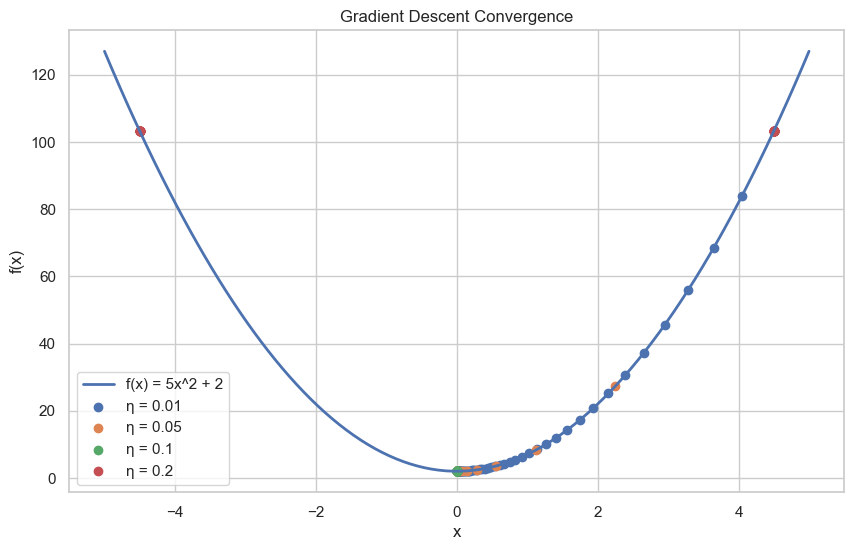
\includegraphics[width=16cm]{output.png}

From the above graph, the range of values that $\eta$ (learning rate) can take for gradient descent to converge to the minimum from any starting point is between $0$ and $0.2$ $(0 < \eta < 0.2)$.

Here's results from the different values of $\eta$:

\begin{itemize}
  \item $\eta = 0.01$: This value yields the slowest convergence. Though it eventually reaches the minimum, its small step size makes the descent very gradual.

  \item $\eta = 0.05$: This value offers a good balance between speed and stability. It converges to the minimum faster than $\eta = 0.01$ while still maintaining smooth descent.

  \item $\eta = 0.1$: This value converges even faster than $\eta = 0.05$, but the descent path appears slightly more aggressive.

  \item $\eta = 0.2$: This represents the highest value for successful convergence. It reaches the minimum quickly, but with potentially larger oscillations around the minimum due to a larger step size.
\end{itemize}

Values of $\eta$ greater than $0.2$ $(\eta > 0.2)$ are not shown on the graph, because a significantly large step size might cause the algorithm to overshoot the minimum and oscillate back and forth around it, ultimately failing to converge. Therefore, the range of $0 < \eta < 0.2$ ensures that gradient descent converges to the minimum from any starting point while balancing convergence speed and stability and the suitable learning rate for this problem is $0.05.



\end{list}
\end{document}  


